\chapter{Mon stage}
\label{sec:unchapitre}

Lorsque j'ai répondu à l'offre de stage, il avait initialement prévu que je produise une newsletter ainsi que trois vidéos sur trois APIs différentes qui sont :

\begin{itemize}
    \item Gat'Ape/Okapi
    \item Zbus
    \item Valkey
\end{itemize}

Cependant, aux vues de mon avancement et de l'intérêt suscité par les vidéos produites, j'ai accepté de travailler sur trois autres projets qui sont :

\begin{itemize}
    \item Explication des difficultés liées à la création et à la publication d'APIs avant l'arrivée du cloud au sein d'Orange
    \item Présentation des avantages du travail en DevOps
    \item Promotion de PnS.com
\end{itemize}

Les vidéos traitant des APIs se devaient d'être vulgarisées et simple à comprendre étant donné qu'elles pourraient être destinés à un public très vaste. Chaque vidéo se doit d'être compréhensible par un programmeur, un manager ou un commercial par exemple. La principale difficulté est de devoir vulgariser un maximum tout en gardant un maximum de précision pour qu'elles restent pertinentes pour les personnes les plus techniques. La diffusion de ces vidéos peut se faire pour montrer les dernières avancées au sein de la SDFY, ou encore pour promouvoir un produit, ou le proposer à des clients en tant que nouvelle solution. \\

En revanche, l'approche pour les 3 autres vidéos est totalement différente, elles s'adressent à un public ciblé et ont principalement un but promotionnel. Deux de ces vidéos ont été réalisées pour un événement particulier. \\

Dans les points suivants, nous allons développer le contexte et la production de chaque vidéo.


\section{Gat'Ape/Okapi}

\subsection{Contexte}
Gat'ape/Okapi est une API faisant partie de l'écosystème PnS.com qui permet d'exposer, de s'autentifier et de sécuriser les APIs de cet écosystème. Gat'ape et Okapi ont deux fonctions bien distintes.\\

Okapi est le système d'authentification qui va permettre la connexion aux autres APIs. Okapi est basé sur le couple Oauth2/Kerberos qui va permettre une identité indépendante à chaque entité tout en offrant un sytème d'authentification unique (SSO) qui va permettre à l'utilisateur d'accéder à plusieurs applications en ne s'authentifiant qu'une seule fois. Cette authentification repose sur un système de clé secrète et de jeton. Il est à noter que des options de sécurité plus complexes sont aussi disponibles.\\

Gat'ape quant à elle est la passerelle qui va permettre d'exposer les APIs, c'est à dire, des les rendre visible à d'autres utilisateurs pour qu'ils puissent s'y connecter. Gat'ape va pouvoir offir un conrôle d'accès et un contrôle de traffic permettant de réguler le flux des utilisateurs. Gat'ape est également responsable  de l'authentification et de la sécutité lors de la consommation par Okapi. En plus de cela, gat'ape est également scalable, c'est à dire qu'elle va pouvoir maintenir son activité et sa performance même lors d'une forte demande.\\

Dans les faits la connexion grâce à Gat'ape/okapi se passe comme suit : 
L'application qui vient se connecter possède une clé secrète. Cette clé secrète est envoyée à Okapi. Lors du traitement, Okapi va renvoyer un jeton d'authentification unique au consommateur ainsi qu'un digest. Ceci est la phase d'authentification.  Ce digest est ensuite envoyé du consommateur vers Gat'ape. Si le digest est valide, le consommateur va envoyer le jeton précédemment obtenu vers l'API à laquelle il souhaitait se connecter. L'API va à son tour vérifier le token puis le renvoyer ainsi que les informations demandées par le consommateur. Ces informations luis seront transmises via Gat'ape. Si une de ces vérifications de token échoue, le protocole recommence un envoi de token. L'opération peut ainsi être réitérée un certain nombre de fois sans avoir à se ré authentiier. Cette durée de vie (TTL) est paramétrable.

\begin{figure}[htp]
  \centering
  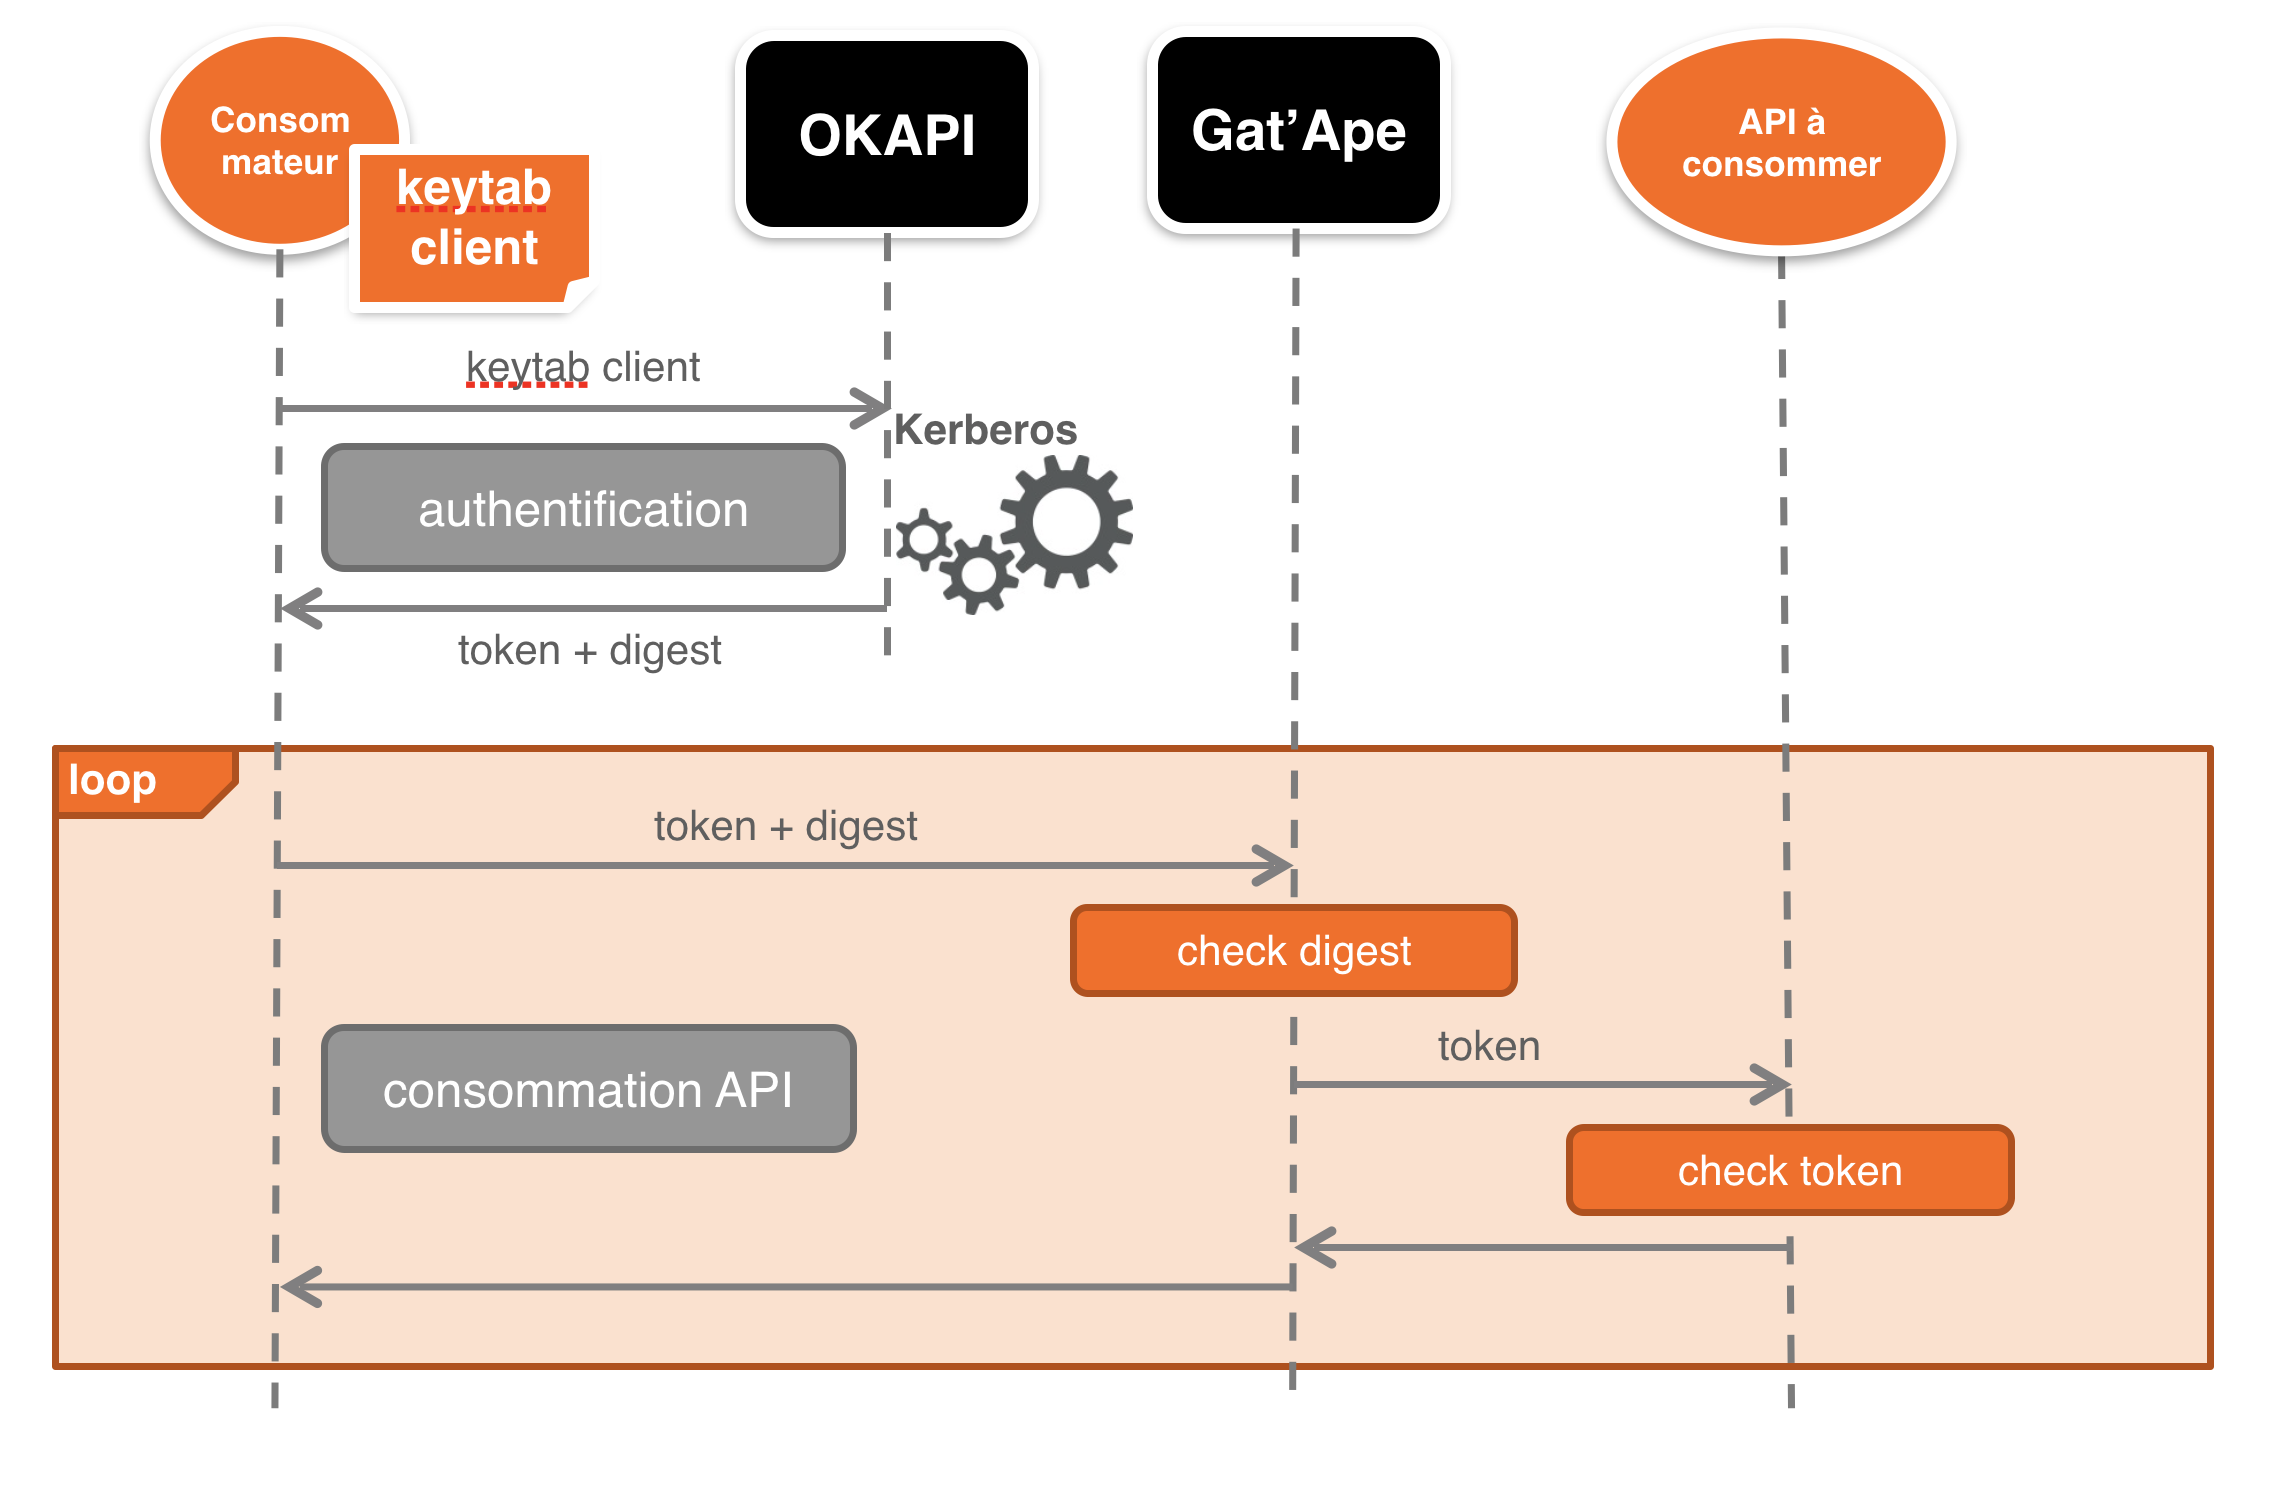
\includegraphics[width=15cm]{images/gao/gao1}
  \caption{Fonctionnement de Gat'Ape/Okapi.}
  \label{fig:une-autre-image}
\end{figure}



\subsection{Production}



\section{Zbus}

\subsection{Contexte}

\subsection{Production}



\section{Valkey}

\subsection{Contexte}

\subsection{Production}

%%% Local Variables: 
%%% mode: latex
%%% TeX-master: "isae-report-template"
%%% End: 